\chapter{Herramientas utilizadas}
\label{cap:capitulo3}

En este capítulo se describen las herramientas y tecnologías utilizadas para la elaboración de los 2 ejercicios de Unibotics. Su desarrollo ha abarcado varios campos: programación del comportamiento autónomo del Robot mediante ROS 2, desarrollo de la imagen docker RADI versión 4 de Unibotics, uso hardware específico para el robot Turtlebot 2 real, etc.\\

\section{ROS (Robot Operating System)}
\label{sec:ros}
ROS (Robot Operating System) es un middleware que ayuda a la programación de robots a través de varias librerías y herramientas desarrolladas por la comunidad de software libre. Entre las ayudas que proporciona este framework están la abstracción del hardware, controladores de dispositivos y de herramientas de visualización entre otros.\\

\subsection {ROS y ROS 2}
\label{sec:ros_versions}
La primera versión de ROS salió en 2010 (ROS Box Turtle) y a partir de ahí han ido surgiendo nuevas versiones siendo la actual y estable ROS Noetic.\\

El funcionamiento de ROS se basa en un sistema centralizado donde un nodo principal se encarga del intercambio de información entre otros nodos del que forma la aplicación, los cuales se comportan como publicadores o suscriptores, permitiendo así, ejecutar en paralelo varios procesos que se dedican a subtareas específicas del robot. De esta forma, por ejemplo, se puede tener un nodo encargado de la recogida de datos de la cámara y otro que comande velocidades dependiendo del resultado del procesamiento que se ha obtenido del nodo de visualización.\\

\begin{figure} [h!]
  \begin{center}
    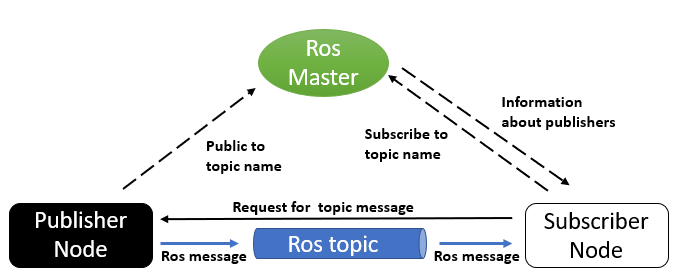
\includegraphics[width=15cm]{imagenes/ros_master_communication.png}
  \end{center}
  \caption{Comunicación del nodo Master con los nodos Intermedios (ROS)}
  \label{fig:ros_master_comunicación}
\end{figure}\

De manera paralela, ha ido surgiendo ROS 2 que es una versión en auge que incorpora nuevas características y novedades en cuanto a su uso. Al igual que en ROS se basa en publicadores y suscriptores, sin embargo, no usa un nodo maestro, y posee mecanismos de seguridad para asegurar la autenticación de los nodos y la integración de los mensajes. La versión mas reciente y estable es \textbf{ROS Foxy}. Es la distribución usada en este proyecto.\\

Los lenguajes de programación que soporta tanto ROS como ROS 2 son C++ y Python.\\

\subsection{URDF}
\label{sec:urdf}

\textbf{URDF (United Robotics Description Format)} es un lenguaje de marcado para describir robots (eslabones, uniones, jerarquías, modelo visual, modelo de collisión, modelo inercial, controladores, etc) que usa la gramática de XML. Se utiliza tanto para robots reales como simulados.\\

La sintaxis sigue la siguiente \textbf{regla}: El robot se divide en su mayoría en eslabones (links) y uniones entre eslabones (joints), de manera que se forma un árbol jerárquico desde un eslabón principal (root) hasta los eslabones terminales.\\

Para definir un link hay que proporcionarle su modelo visual (<visual>), su modelo de colisión (<collision>) y su modelo inercial (<inertial>). Después se define el joint que une el eslabón que hemos definido con otro mediante una jerarquía de padres e hijos.\\

\begin{code}[h]
\begin{lstlisting}[language=XML]
<?xml version="1.0"?>
<robot name="simple_cube">
	<link name="base_link">
		<visual>
			<origin xyz="0 0 0"/>
			<geometry>
				<box size="1.0 1.0 1.0"/>
			</geometry>
		</visual>
		<collision>
			<origin xyz="0 0 0"/>
			<geometry>
				<box size="1.0 1.0 1.0"/>
			</geometry>
		</collosion>
		<inertial>
			<origin xyz="0 0 0" /> 
			<mass value="1.0" />
			<inertia  ixx="1.0" ixy="0.0"  ixz="0.0"  iyy="1.0"  iyz="0.0"  izz="1.0"/>
		</inertial>
	</link>
</robot>
\end{lstlisting}
\caption[Ejemplo de código URDF: Definición de un cubo]{Ejemplo de código URDF: Definición de un cubo}
\label{cod:codigo_urdf}
\end{code}

\subsection{XACRO}
\label{sec:xacro}

XACRO (TODO)

\section{Lenguajes de Programación}
\subsection{C++}
\label{sec:c++}

C++ es un lenguaje de programación diseñado en 1979 de Bjarne Stroustrup. Deriva del lenguaje C, y destaca principalmente porque incorpora el paradigma de la Programación Orientada a Objetos (POO). Además, incorpora una gran cantidad de nuevas librerías para facilitar la programación entre ellas las librerías estandar y STL (Standard Template Library).\\

Muchos paquetes de ROS se programan con C++ debido a la gran cantidad de posibilidades que presenta este lenguaje para desarrollar Plugins, Behavior Trees, Máquinas de Estado, etc.

\subsection{Python}
\label{sec:python}

Python es un lenguaje de programación interpretado que destaca por su legibilidad, facilidad y soportabilidad a la programación Orientada a Objetos. Posee características particulares que lo diferencian de otros lenguajes de programación como puede ser el uso estricto de indentación en bloques de código.\\

La infraestructura de Unibotics y de Robotics Academy están programadas en Python

\subsection{Javascript}
\label{sec:javascript}

Javascript es un lenguaje de programación interpretado que destaca por ser utilizado en el lado del cliente, en el Frontend de una página web que lee el navegador. Con Javascript podemos crear páginas web dinámicas a través de la definición de eventos que provocan resultados en el Backend (si tiene) o en la propia estructura HTML. Javascript puede usarse para más cosas: Websockets, Canvas, Animaciones, etc...\\

En las plantillas web de Robotics Academy se usa Javascript para comunicar los eventos del exercise.html con exercise.py

\section{Lenguajes de Marcado}
\label{sec:html}

HTML (TODO)

\section{CSS}
\label{sec:css}

CSS (TODO)

\section{Docker}
\label{sec:docker}

Docker (TODO)
